\subsection{Routing Control Platform (RCP)}\label{sec:arch}
Building on the principles from Section~\ref{sec:principles}, this
subsection proposes a {\em Routing Control Platform} (RCP), which
separates the control-plane logic from the routers that forward packets.
We describe RCP as a single, logically-centralized entity in each
domain. This centralized function must actually be implemented in a
reliable, physically distributed fashion to avoid introducing a single
point of failure and ensuring robust route distribution.  We believe
that existing distributed systems techniques may be applicable; this
dissertation does not address this issue in detail, but we briefly
discuss it in Section~\ref{sec:weaknesses}.

We describe RCP in terms of three phases: (1) controlling routing
protocol interactions by replacing iBGP route reflection with RCP, (2)
gaining flexibility over route selection by making RCP the
endpoint of all eBGP sessions with neighboring ASes, and (3) enabling
changes to interdomain routing by using RCPs, rather than routers, to
exchange routes between ASes using eBGP or some new protocol.
%
By describing RCP in terms of three stages, we demonstrate that RCP is
incrementally deployable {\em within an AS\/} and, more importantly,
provides significant benefits to an individual AS even if other ASes
have not deployed RCP.  In addition to being steps of incremental
deployment, each phase provides  new functionality while
remaining  backwards compatible with BGP.  
%RCP simplifies the
%operation of interdomain routing within individual ASes, regardless of
%whether other ASes deploy RCP. However, RCP's full potential is only
%realized when it is completely deployed by a group of interconnected
%ASes or throughout the entire Internet.
%The rest of this subsection describes these three modes of deployment in
%further detail.  For each stage, we describe the changes that must be
%made to the way that BGP is {\em configured}, as well as how each stage
%makes reduces complexity and enables innovation.
%Table~\ref{ref:phases} summarizes the architectural changes at each
%phase of evolution, as well as new features and functionality that are
%enabled at each phase.

%% \begin{figure}
%% \centering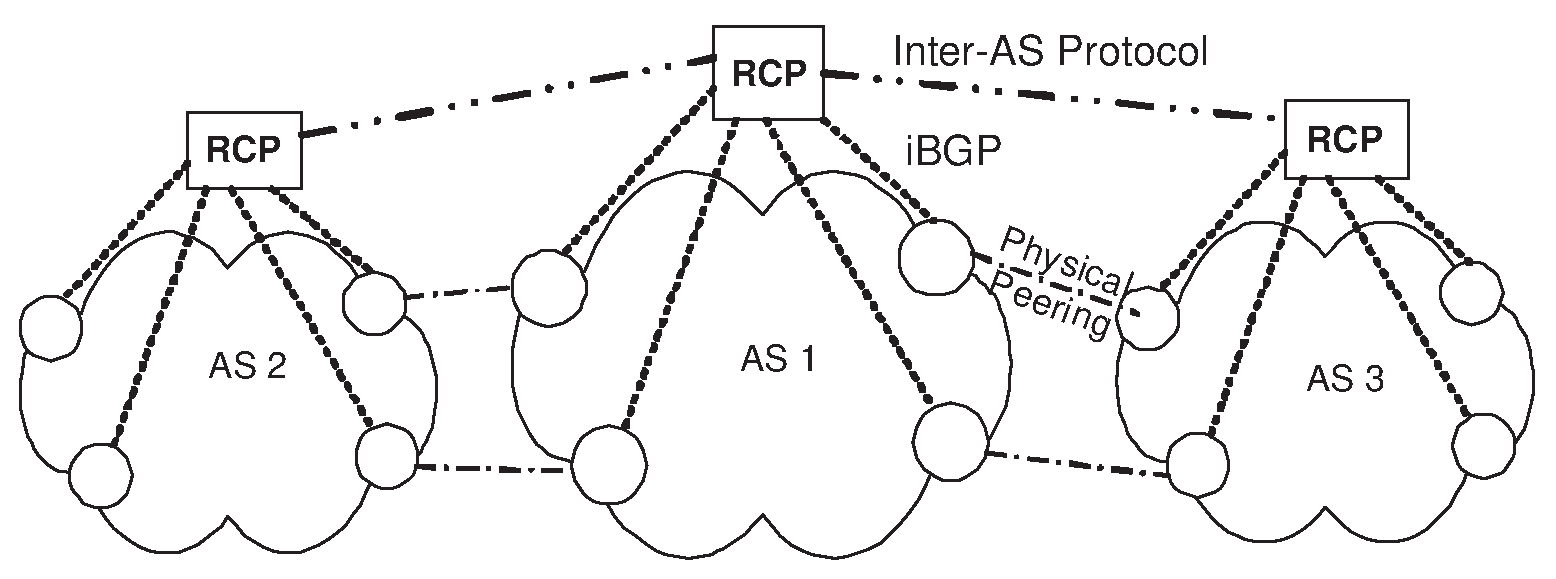
\epsfig{file=rcp/figures/interas.eps, width=\linewidth}
%% \caption{An extensible routing platform for the Internet.}
%% \label{fig:interas}
%% \end{figure}


%%%%%%%%%%%%%%%%%%%%%%%%%%%%%%%%%%%%%%%%%%%%%%%%%%%%%%%%%%%%

\paragraph{Control Over Protocol Interactions}\label{sec:feamster:fdna2004_ibgp}


%% note: already exists a monitoring infrastructure.  now we're going to
%% let the monitor "talk back" 
%% A route authority must have sufficient information about the state of
%% the network from the perspective of its clients to make the correct
%% decision for each client.  The route authority acts as a proxy for each
%% of its clients; thus, to make the same decision that the client would
%% have made in a full-mesh configuration, the authority must have access
%% to all of the information that the client would have used to make the
%% same routing decision in a full mesh (\eg, IGP path costs from that
%% client to a network egress point).

The first phase of RCP deployment, shown in Figure~\ref{fig:ibgp_only},
involves only minor changes to the iBGP {\em configuration\/} inside
an AS.  
% Monitoring the IGP
First, RCP monitors the IGP to
maintain an accurate, up-to-date view of the IGP topology; previous
work explains how to monitor an IGP without disrupting the operation
of the network~\cite{Shaikh2004}.
Next, instead of having routers propagate eBGP-learned routes through
an iBGP hierarchy, a router sends its best route for each eBGP-learned
destination to RCP via an
iBGP session.
% Making the decisions
Finally, RCP computes a route for each router and conveys that route via
the iBGP session. 
% It's not too bad
Using an RCP does not require any changes to the routers themselves
(aside from the configuration of iBGP sessions to RCP) or the
configuration of routers in other ASes.  Many ISPs already deploy a
monitoring infrastructure to keep track of network state and routing
protocol behavior.  At this stage, RCP is essentially an IGP and BGP monitoring
infrastructure that also {\em controls} route selection.


\begin{figure}
\centering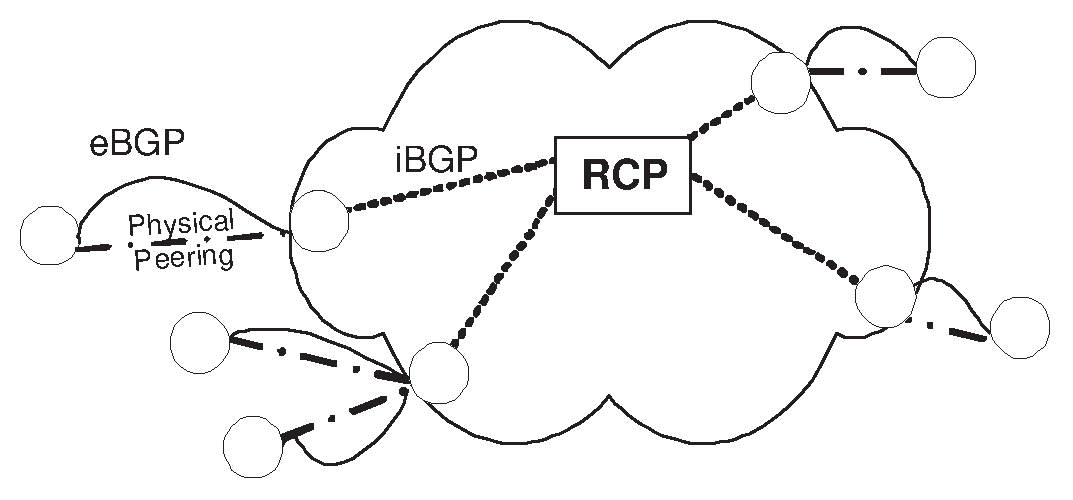
\epsfig{file=rcp/figures/ibgp.eps, width=0.6\linewidth}
\caption[The first phase of RCP deployment]{The first phase replaces the
pairwise iBGP sessions between  
routers with iBGP sessions to RCP.  RCP uses knowledge about the
IGP topology and the best routes from each border router to
make routing decisions on behalf of each router.  RCP distributes the
path assignment to the routers via iBGP.}
\label{fig:ibgp_only}
\end{figure}


This stage of RCP closely resembles an architecture based on route
reflection~\cite{rfc2796}, but, unlike route reflectors,
RCP can return a {\em different\/} best route to each router.  For
example, RCP could compute the route that each router would have
selected in a full-mesh iBGP topology.
%, which computes the same routes
%as a full-mesh configuration (unlike
%a route-reflector hierarchy).  
RCP also offers more
flexibility than route reflection because it is not
limited to emulating a full-mesh iBGP scenario: RCP could
intentionally select other routes to control the interactions between
iBGP and the IGP.
% not a route server
RCP may also appear similar to previous work on route
servers~\cite{rfc1863} that forward {\em all\/} BGP-learned routes to
their clients, but, because it forwards only {\em one\/} route to each
client, RCP remains backwards compatible with BGP and enables
customized path selection.

In the rest of this paragraph, we present several examples to 
show how this stage of RCP deployment simplifies important network
management tasks. 

{\bf Enforceable correctness constraints and invariants.}  With
complete knowledge of the iBGP and IGP topologies, RCP can 
enforce a clean separation of routing layers.  
%For example, as we pointed out in Section~\ref{sec:principles},
%interactions between iBGP and IGP can result in incorrect routing if
%certain sufficient conditions are not satisfied.  Currently, operators
%must check these conditions manually or with an external configuration
%checker~\cite{feamster03:verify}.  Of course, the RCP could examine
%the routing protocol configuration and check these sufficient
%conditions, but, because the RCP {{\em controls} the routing decisions
%for the routers in the AS, it can directly {\em enforce} correctness
%constraints.  For example, persistent forwarding loops can result if
%the routers along an IGP path do not select the same BGP
%route~\cite{Dube99}.
For example, RCP can ensure that each router along a forwarding
path selects the same best BGP route for a destination prefix, which
prevents the forwarding loops and protocol oscillations that 
can arise in conventional iBGP configurations~\cite{Dube99,Griffin2002}.
%
RCP can also be useful for detecting persistent oscillations caused by
the MED attribute~\cite{Griffin2002b}, which occurs because routers do
not have a total ordering over the set of candidate routes.  With a complete
view of the best routes from each border router, RCP can recognize
when each router would not have a single, consistent ordering and
can force the system into a stable path assignment. 

%% {\bf Improved routing during convergence.}  Because correct, loop-free
%% routing within an AS depends on consistency between iBGP and IGP routes,
%% forwarding loops can also result as a result of either iBGP or IGP
%% convergence.  For example, two routers may agree on an egress router for
%% a global destination.  If one of those routers hears a withdrawal for
%% that exit point before the other, the router that first hears the
%% withdrawal could select an alternate route that forwards packets towards
%% the router that has not yet heard the withdrawal and is still using the
%% old exit point.  Such a situation could cause unnecessary transient
%% forwarding loops during convergence.  By removing the complexity of
%% route propagation from the routers themselves (Principle~1), the RCP can
%% control the propagation convergence-related routing changes to minimize
%% these temporary inconsistencies.

{\bf Avoiding unintentional hot-potato routing changes.}  Small
changes in the IGP topology (\eg, due to traffic engineering,
failures, or planned maintenance) can trigger large, unnecessary
shifts in eBGP routes because of BGP's ``hot potato'' routing
behavior~\cite{teixeira2004b}.  RCP can allow a network operator to add
or remove internal links, or modify the IGP costs, without worrying
about the side effects on BGP path selection.  By controlling the path
selection for each router, RCP can force routers to continue using an
egress point even when a link failure or small IGP cost change makes
another egress point become slightly ``closer''.  (RCP must take care
to ensure that each router along the forwarding path to the egress
point for that router continues to pick the same egress point.)  In
addition to avoiding unnecessary traffic shifts,
% and BGP convergence delays within an AS, 
preventing these abrupt routing changes improves global
routing stability by reducing the number of eBGP routing changes
propagated to downstream neighbors.

{\bf More flexible traffic engineering.}  RCP can
{\em intentionally\/} change the egress point for a router to move
traffic to a lightly-loaded edge link or a less congested downstream
path.  This approach allows the AS to balance the traffic load without any
changes to the import policies on eBGP sessions or the IGP link costs.
In addition to controlling the egress point, RCP could
dictate the entire forwarding path through the AS rather
than relying on the IGP.  For example, RCP could send a router a
BGP route with a ``next hop'' that corresponds to an immediate
neighbor in the IGP topology, which would cause that router to create a
forwarding table entry that maps the destination prefix to the
outgoing link connecting directly to the neighboring router.  
This
kind of fine-grained control is useful for planned routing changes.
RCP could make these routing
changes incrementally (\ie, one router at a time) to avoid creating transient
forwarding loops during convergence.
%For example, the RCP could pin a fixed path through a sequence of
%routers in an AS by ensuring that those routers were always assigned
%the same exit point for a destination (exit-point tunneling).  If an
%AS already performs intra-AS routing with tunneling (\eg, with MPLS),
%RCP can simplify path selection further---once label distribution has
%established paths, RCP can distribute traffic flow across the AS
%simply by assigning labels at ingress routers.

%The RCP could also assign routes to a destination with the next-hop
%attribute for each router set to the next {\em intra-AS hop} within that
%AS, rather than to that of the exit point (intra-AS ``hop-by-hop'' routing).
%Using hop-by-hop routing with RCP has several advantages.  First,
%because the intra-AS path is explicitly encoded in the iBGP route, each
%iBGP hop can potentially be only a single IGP hop; this feature
%decouples iBGP and IGP.  Second, this decoupling makes traffic
%engineering and network management much more flexible, because operators
%can establish intra-AS paths using the RCP without worrying about how
%those paths will be affected with IGP paths change.

%% {\bf More expressive backup policies.}  Ability to express new policies,
%% such as those involving multihoming and backup (Rekhter's RFC on
%% multihoming and aggregation, ideas about failure detection/health
%% monitoring).  Something about health monitoring here; knowing when to punch
%% holes, etc. requires knowing whether the eBGP link has failed, or
%% whether some iBGP link has failed.


%% {\bf XXX should have an example here XXX} Each client should be able to
%% select the route that it would have selected in a full-mesh
%% configuration.  The route or routes that a client learns via the
%% intra-AS routing protocol should always include the route that the
%% client would have selected in a full-mesh iBGP configuration.  What
%% problems go away with tunneling?  Forwarding path inconsistencies {\em
%% only} (deflection and forwarding loops).  Rest of the problems remain.


%% There is a broad spectrum of possible solutions that could simulate a
%% full mesh, many of which would involve changing the format of routing
%% messages or the behavior of BGP.  Because a new architecture should be
%% interoperable with today's routers, the architecture we propose does not
%% make any changes to either the BGP messages or the BGP decision process
%% on the clients (\ie, production routers).  Our architecture creates a
%% new entity, a {\em route authority}, that behaves differently than a
%% BGP-speaking router does today, but the {\em interface} to the authority
%% (\ie, the messages exchanged between the authority and other routers)
%% looks exactly as BGP does today. Section~\ref{sec:arch_details}
%% discusses the solution we propose in greater detail.

%% {\em Change RRs to advertise all routes (or all equally good routes)}:
%% cite~\cite{Basu2002}.  however, primarily a problem of backwards
%% compatibility and overhead.


\paragraph{Network-Wide Path Selection and Policy}
\label{sec:feamster:fdna2004_ebgp}

\begin{figure}
\centering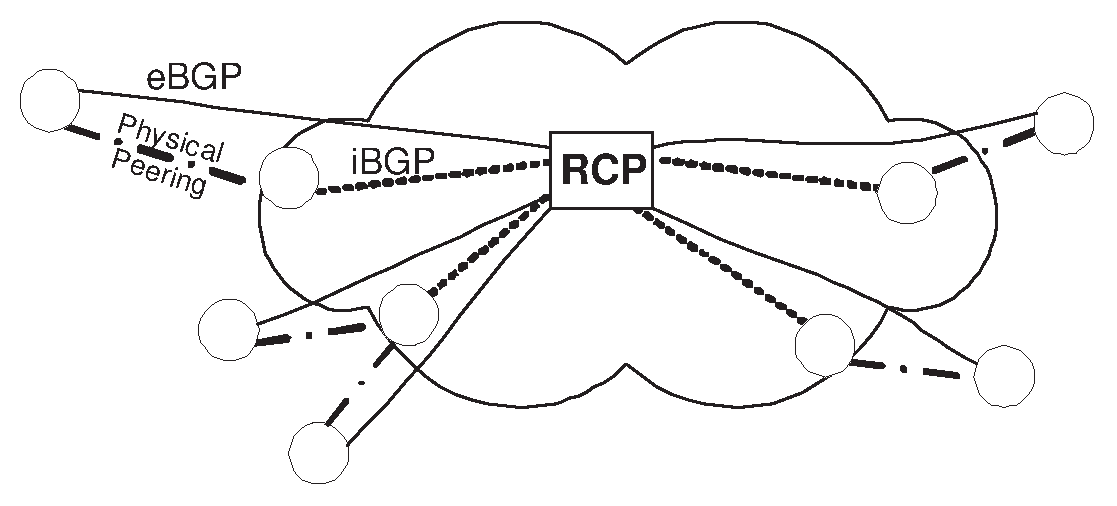
\epsfig{file=rcp/figures/ebgp.eps, width=0.6\linewidth}
\caption[The second phase of RCP deployment]{The second deployment phase
of RCP operates in a similar manner 
  as the first phase, but now RCP itself has eBGP sessions
  to routers in other ASes, rather than relying on border routers
  to learn routes from other ASes and apply local policies.}
\label{fig:ebgp}
\end{figure}


In the first deployment phase, the AS's border routers continue to
exchange routes with neighboring domains.  The AS's border routers still apply
local import and export policies and forward a single best route for
each prefix to RCP.  In the second stage, RCP exchanges routes
directly with the border routers in other ASes, as shown in
Figure~\ref{fig:ebgp}.  Neighboring ASes must modify the
configuration of their eBGP sessions to peer with RCP, rather than
with individual routers.\footnote{Each router on the path
  between RCP and routers must also have routes for both endpoints.
These routes can be established by injecting routes for the endpoints
into the routing protocol or by configuring static routes.}
This change only involves changes to the router {\em configuration}, not the
underlying hardware or software, and it
offers significant benefits because (1)~RCP has access to {\em all\/}
routes learned via eBGP from other ASes, (2)~all routing policies
for the AS are applied directly at the RCP, and (3)~the border routers do
not need any BGP configuration beyond their iBGP session to RCP. 
This phase of RCP significantly simplifies network management.

{\bf Simpler routing configuration.}  With all of the eBGP-learned
routes in one place, the configuration of the routing policies can
reside entirely at the RCP.  Rather than using BGP communities to tag
routes at one router to ensure the correct handling at another router,
RCP can classify and select the routes itself.  For example, suppose
eBGP routes learned from one peer should not be advertised to another.
RCP could maintain a local registry of peer and customer AS
numbers and ensure that routes where the neighboring AS is a peer AS
are not advertised via eBGP sessions to other peer ASes.  In today's
routing infrastructure, the auxiliary information about peer and
customer ASes would be expressed indirectly (\ie, in the import
policies that tag the routes learned on certain eBGP sessions and
export policies that filter routes based on these tags).  With the RCP
performing all routing decisions, this type of decomposition is unnecessary.

{\bf Network-wide traffic engineering.}  In the second phase, RCP has
access to {\em all\/} of the eBGP-learned routes, not just the best
paths selected by the border routers.  With complete control over the
selection of paths, RCP can disregard the unwieldy BGP
decision process.  RCP can influence
the routing decisions of various routers directly, without 
meddling with local preference settings at individual routers.  Rather
than generating complex import policy rules that manipulate the
local preference attribute, RCP could explicitly decide which path
each router should select for any destination prefix.  In
addition to comparing the eBGP-learned routes, RCP could base routing
decisions on
auxiliary information such as measured traffic volumes, performance
statistics (\eg, observed packet loss), and commercial
relationships with neighboring domains (\eg, the pricing model).
%Directly incorporating these metrics into the
%routing protocol is a more appealing way to engineer
%the flow of traffic in the network than trying to find a suitable
%setting of distributed configuration parameters~\cite{Feamster2004}.
%It could, for example, decide to ignore AS path length as a step in
%the decision process, or group routes with different AS path lengths
%into the same equivalence class to assist with traffic
%engineering~\cite{Feamster2003e}.

{\bf Intelligent route-flap damping.}  Many BGP update sequences
are caused by routers performing ``path exploration'': upon learning of
a route's 
withdrawal from a neighboring AS, a router will readvertise its second
best path until it receives the corresponding withdrawal for that path, and
so on.  RCP can prevent route-flap damping from discarding an
otherwise stable route.  Rather than having routers implement route-flap
damping independently, RCP could damp routes on behalf of routers in
the AS based on a network-wide view of the eBGP-learned routes.
Additionally, RCP could determine when advertisements appear to stem
from path exploration and use this information to delay readvertisement,
thus preventing routers in neighboring ASes from receiving a flurry of
transient advertisements during path exploration.

{\bf Coalescing routing table entries with customized aggregation.}
Networks often advertise multiple subnets in the same address block to
balance the flow of traffic over several incoming links, which can
lead to large routing tables and a larger number of BGP update
messages.  An individual router cannot typically safely aggregate
subnets with the same next-hop, because another router in the AS may
need to treat the subnets 
differently.  As 
such, operators are often conservative in aggregating routes to
prevent unintentional blackholes and forwarding loops.  Giving RCP
control over which BGP routes are sent to each router permits
more aggressive aggregation.  For example, if RCP
discovers that the BGP routes for 12.1.2.0/24 and 12.1.3.0/24 at some
router will use the same outgoing interface, it can send a single
12.1.2.0/23 route to the router, which can substantially reduce the
memory requirements for the routing and forwarding
tables.\footnote{An individual router can coalesce subnets when
constructing its local {\em forwarding\/} table~\cite{draves99}, but
this approach does not reduce the size of the BGP routing table or the
number of BGP update messages.}  (Note that RCP can send an
aggregated route to a router even if the two initial routes have {\em
different} AS paths, since the individual routers no longer act on
this information.)  This technique can also reduce the
number of BGP updates, since
many BGP routing changes affect attributes such as AS path, community,
and MED that do not affect forwarding.

%ASes often advertise more specific prefixes to load balance incoming
%traffic; for example, an AS might split a ``$/19$'' prefix into two
%$/20$ prefixes and advertise each smaller prefix on a different link.
%An AS might also divide its prefix into smaller prefixes according to
%geography.  These more specific prefixes can provide ISPs more
%efficient routes to destinations, but they also inflate routing table
%size.  For example, the CIDR report suggests that more aggressive
%aggregation for prefixes that have the same AS paths could reduce
%routing table size by about 40,000 prefixes~\cite{www-cidr}.  An AS's
%RCP can recognize when a router in the AS would select the {\em same}
%route for two contiguous smaller prefixes and aggregate the two
%smaller prefixes into a single routing table entry on that router.

%{\bf Diagnostics.}
%% XXX Punt this paragraph?  Too confusing?
%% An RCP can also enable an AS to perform better diagnostics by providing
%% all eBGP-learned routes in a centralized location.  For example, an AS
%% typically wants to verify that a neighboring AS with which is has a
%% commercial ``peering'' relationship is advertising routes with
%% equally good attributes at all peering locations between the two ASes.
%% Checking this constraint in today's routing architecture is challenging
%% because the routes that one AS advertises to another are distributed
%% across multiple routers.  
%% %Monitoring the best routes from these routers
%% %via iBGP is difficult because some of these routers may choose best
%% %routes from different peers.  Looking at routing table dumps will show
%% %what routes each router hears, but because of the asynchrony, mismatches
%% %in routes as seen in routing tables may reflect inconsistencies due to
%% %timing, rather than actual inconsistent advertisement.  
%% An RCP makes
%% these problems go away because all eBGP routing information is
%% maintained at a logically centralized place.


\paragraph{Redefinition of Inter-AS Routing}\label{sec:interas}

%In the second phase, eBGP is a legacy routing protocol for exchanging
%BGP routes with ASes that do not have RCPs of their own.  
In the third
phase, multiple ASes with RCPs can exchange interdomain routing
information directly through their RCPs, as previously shown in
Figure~\ref{fig:interas}. As in the first
two phases, RCP makes routing decisions on behalf of the
routers in its AS.  
%In the simplest scenario, multiple ASes belonging
%to the same institution use RCPs to coordinate their routing
%decisions, a provider's RCP can coordinate with a customer's RCP to
%offer new network services.  
%Ultimately, we envision each AS having
%its own RCP.  
RCP could simply use eBGP to exchange routing
information, but exchanging routes with eBGP is not strictly necessary.
RCP could also enable ASes to better coordinate when 
diagnosing routing problems and selecting paths.

{\bf Better network diagnostics and troubleshooting.}  RCP could
provide diagnostic information to a neighboring AS (or even remote ASes)
upon request.  Network operators regularly send email to
mailing lists (\eg, NANOG) to ask other operators about possible
reachability problems and diagnose problems as they arise.  With RCPs
deployed in many ASes, the collection of RCPs could be treated as a
distributed database of routing information, where each AS maintains a
portion of and provides a query interface to that
information~\cite{Teixeira2004}. 
An AS
could allow other ASes to query the routes that it has learned from
other ASes for debugging (\ie, using RCP query interface as a
sort of master ``looking glass'' server for the entire AS) or
verification~\cite{Feamster2003b} (\eg, verifying an AS path by
asking other ASes along that path if they have learned corresponding
route).
%
Of course, the diagnostic information need not be limited to BGP
data.  For example, RCP could maintain information
about intra-AS topology changes, link congestion, and performance
statistics to help explain disruptions in end-to-end performance.

{\bf New interdomain routing protocols.}  RCP
enables a variety of proposals for fundamental changes
to interdomain routing.  Recent proposals have advocated
modifying the way the interdomain routing protocol selects and
propagates routes. For example, a new routing protocol could attach
prices to advertised routes~\cite{Feigenbaum2002} or explicitly
support inter-AS negotiation to select the routes~\cite{mahajan2005}.
RCPs could also base their routing decisions on measured
end-to-end performance, as proposed in work on overlay
networks~\cite{Andersen01} and even make this performance information
available to end-host overlays through appropriate
interfaces~\cite{Nakao2003}.
%
Other proposals have suggested ways to improve security by performing
path authentication~\cite{Subramanian2004} or origin
authentication~\cite{Aiello2003}.  Until now, many of these proposals
have had no feasible deployment path because they require fundamental
protocol changes and would not be backwards compatible with the
installed base of routers.  RCP allows the deployment of new routing
protocol changes without modifying or replacing the existing infrastructure.

%Pairs of ASes must sometimes coordinate their policies to achieve
%certain traffic engineering tasks.  In Section~\ref{sec:principles}, we
%described, the complications involved in expressing bilateral
%interdomain routing policies such as backup and load balance.  RCP
%could simplify this type of policy negotiation by (1)~allowing
%high-level policies like backup to be negotiated in-band (\ie, in the
%routing protocol itself) and (2)~allowing complex traffic policies to be
%implemented without indirect, low-level tweaks of routing protocol
%attributes.

%In addition to previously proposed protocol alternatives, an RCP-based
%routing architecture enables other types of fundamental changes to the
%routing protocol.  For example, the RCP could exchange performance
%information (\eg, path level performance information that overlays
%currently perform~\cite{Andersen01}, information about resource
%availability, etc.) that could help inform routing decisions.
